\chapter{Fundamentos de la Inteligencia Artificial y sus herramientas}\chaptermark{Fundamentos de la IA y herramientas}\pagestyle{mypagestyle}

	En este capítulo se abordará una breve introducción al campo de la Inteligencia Artificial, comenzando desde su historia a lo largo del tiempo para contextualizar, pasando por entender los fundamentos de lo que busca lograr, y comentando alguna herramienta matemática que será de utilidad y que en ciertos casos causa confusiones. 

	\section{Breve historia de la Inteligencia Artificial}
	
		Ya desde hace varias décadas, se planteaba la posibilidad de que las máquinas fuesen capaces de realizar tareas diferentes a meros cálculos. La persona que realizó dicha afirmación fue la matemática Ada Lovelace, que en 1842 programó el considerado primer algoritmo. No fue hasta bastantes años más tarde en 1956 cuando se celebra la Conferencia de Darmouth por los hoy considerados padres de la IA, en la que se propone estudiar la Inteligencia Artificial como una ciencia más. En dicha época existían dos corrientes, la simbólica y la conexionista. \\
		
		La primera de ellas se ocupaba de resolver problemas de toma de decisiones y de obtención de conclusiones. Fueron populares los algoritmos de búsqueda y los sistemas expertos. Por otro lado, la corriente conexionista trataba de simular el comportamiento de las neuronas humanas de manera artificial, haciendo que estas neuronas artificiales pudiesen aprender. De aquí surgía el perceptrón que también fue presentado en esta conferencia. Más tarde, entre 1970 y 1980, con el libro de Minsky sobre los perceptrones y sus limitaciones, investigaciones en falso, y bajos recursos, decae el interés y la investigación de la IA. Sin embargo, esta etapa vacía finaliza con la llegada del algoritmo de retropropagación que permitía entrenar redes neuronales multicapa, trayendo consigo infinidad de nuevos proyectos. \\
		
		Años después, avanzados los 2000, se empieza a ver lo poderosos que pueden llegar a ser ciertos modelos de IA al vencer a campeones del mundo en juegos, como a Kasparov en el ajedrez o a Jie en Go. Con la llegada de más y mejores recursos y financiación, hacia 2010 se populariza el uso de redes neuronales para trabajar con imágenes, resolver problemas de clasificación, etc\cite{historiaIA}. \\
		
		Hace diez años surge uno de los modelos de IA con el que se inicia el paradigma que más popularidad está tomando en la actualidad. Este es el de la IA generativa. En 2014 Ian Goodfellow presenta las redes GAN con las que crear nuevos datos, por ejemplo rostros humanos que no existen en realidad, tal y como se muestra en \url{https://thispersondoesnotexist.com/}. Gracias a la IA generativa combinada con modelos de lenguajes, han ido surgiendo en los últimos años herramientas muy poderosas como ChatGPT con la que entablar cualquier tipo de conversación, solicitar información o ayuda para resolver cualquier problema; DALL-E o MidJourney a las que solicitar crear una imagen mediante una descripción por texto, o incluso un vídeo con Sora. 

	\section{Tipos de aprendizaje y problemas}
	
		Al intentar resolver un problema relacionado con el aprendizaje automático, normalmente el primer paso es elegir un modelo que se adapte correctamente al dominio y tipo del problema. De manera ingenua, se puede entender como una especie de caja negra a la que dada una serie de entradas devuelve una serie de salidas que dependen de dichas entradas y una serie de operaciones con respecto a un conjunto de parámetros $\Theta$. Por tanto, para obtener las salidas deseadas para una serie de entradas, el trabajo es encontrar los parámetros óptimos $\Theta^*$ que produzcan dichas salidas. Esto se logra mediante un algoritmo de aprendizaje o entrenamiento, siendo el segundo paso elegir uno acorde al modelo. Normalmente se dispone de dos tipos de aprendizaje, \textbf{aprendizaje supervisado} y \textbf{aprendizaje no supervisado}. Como tercer paso, se debe de medir de alguna manera cómo de bien o mal se está comportando el modelo y el algoritmo, tal y como se estudiará más adelante\cite{Szeliski}. \\
		
		En los problemas de aprendizaje supervisados, se dispone de un conjunto de datos o \textit{dataset}, que contiene los valores de salida deseados para diferentes valores de entrada, normalmente recogiendo situaciones del pasado para poder extrapolar este conocimiento a situaciones del futuro. Los principales problemas que de aprendizaje supervisado son los problemas de clasificación y de regresión. En los \textbf{problemas de clasificación}, se dispone de una serie de clases $C_1, C_2, \hdots, C_n$, y para una serie de valores de entrada $x_1, x_2, \hdots, x_m$, debe decidirse a qué clase pertenece dicha entrada. Un ejemplo sería decidir si un paciente va a sufrir un cierto tipo de cáncer dada su edad, peso, y otras constantes vitales. Algunos de los modelos más populares para llevar a cabo este tipo de tareas son árboles de decisión, máquinas de soporte vectorial, Naïve Bayes, $k-$vecinos, y redes neuronales; siendo estas últimas objeto de estudio en este trabajo. Otro tipo de problema popular a la hora de disponer de datos etiquetados, son los \textbf{problemas de regresión}, que se diferencia principalmente de la clasificación en que en este caso, los valores no son clases (valores discretos) sino valores continuos. Para resolver este tipo de problemas se suelen utilizar regresiones lineales y no lineales (exponencial, polinómica, etc). Un ejemplo de un problema de regresión sería predecir las horas que dormirá una persona dada su edad, horas trabajadas en el día, horas de recreo en el día, etc. \\
		
		Por otro lado, en los problemas de aprendizaje no supervisado no se dispone de los valores de salida esperados para una cierta observación (justo al contrario que en el caso supervisado), pues será trabajo del algoritmo encontrar relaciones y patrones entre los datos proporcionados. En este tipo de aprendizaje también se trata el problema de clasificación, sin embargo, es más común llamarlo \textbf{clústering} o \textbf{segmentación}, pues a priori no se conoce el número de clases y cuáles son, es el algoritmo el que deberá encontrar relaciones entre los datos para determinar esto. Algoritmos populares para realizar esta tarea son $k-$medias (y su variante $k-$medianas), clusterización jerárquica aglomerativa, modelos de mixtura gaussianos, y DBSCAN. Un ejemplo sencillo de este problema es detectar las diferentes regiones y objetos representados en una imagen, pues inicialmente no se conoce el número de regiones u objetos, y deben detectarse todas, asignando cada píxel de la imagen a cada una de ellas. 

	\section{Convolución y correlación cruzada}\label{sec:conv_cc}
	
		Una de las operaciones matemáticas más conocidas y que es más usada al trabajar con señales e imágenes es la llamada convolución, denotada por $\ast$, y dadas las funciones $f(t)$ y $g(t)$, su convolución se define de la siguiente manera. 
		
		$$
		(f \ast g)(t) = \int_{-\infty}^\infty f(\tau)g(t - \tau)\,d\tau
		$$
		
		En este caso se está asumiendo que el dominio de $f(\tau)g(t - \tau)$ es $\mathbb{R}$, lo que permite integrar sobre todo $\mathbb{R}$, de lo contrario, se modifica la definición para integrar solo sobre un intervalo $[a, b]$. En general, esta operación crea una nueva función a partir de otras dos, que indica cómo interactúan entre sí, y que permite aplicar filtros a señales e imágenes. Como se acaba de comentar para el caso de las imágenes, se puede tratar con señales que no dependan únicamente de una variable, pues estas se representan como una función de dos variables $f(u, v)$. En este caso, la convolución queda definida de la siguiente manera. 
		
		$$
		(f \ast g)(u, v) = \int_{-\infty}^\infty\int_{-\infty}^\infty f(\xi, \eta)g(u - \xi, v - \eta)\,d\xi\,d\eta
		$$
		
		Partiendo de las primera definición mostrada, se pueden demostrar algunas propiedades útiles que cumple la convolución\cite{lopez2009metodo}: 
		
		\begin{itemize}
			\item Conmutativa: $f \ast g = g \ast f$
			\item Asociativa: $f \ast (g \ast h) = (f \ast g) \ast h$
			\item Distributiva: $f \ast (g + h) = (f \ast g) + (f \ast h)$
			\item Derivada: $\frac{d}{dt}(f \ast g) = \frac{df}{dt}\ast g = \frac{dg}{dt}\ast f$
			\item Relación con las transformadas de Laplace y Fourier: $\mathscr{L}\{f \ast g\} = \mathscr{L}\{f\} \cdot \mathscr{L}\{g\}$, o lo que suele ser más útil, $f \ast g = \mathscr{L}^{-1}\{\mathscr{L}\{f\}\cdot\mathscr{L}\{g\}\}$, de forma que se puede calcular la convolución en tiempo $\mathcal{O}(n\log(n))$ con el algoritmo FFT\cite{fft}. 
		\end{itemize}
		
		Si bien en las definiciones previas se ha tomado la integral y tanto $\mathbb{R}$ como $\mathbb{R}^2$ como dominios continuos sobre los que calcular la convolución, no se debe olvidar que las imágenes no dejan de ser matrices o funciones de dos variables con un dominio discreto, por lo que se debe presentar una definición adecuada a este caso\cite{Goodfellow-et-al-2016}. 
		
		$$
		(f \ast g)(u, v) = \sum_{i=-k}^{k}\sum_{j=-k}^{k} g(i, j)f(u - i, v - j)
		$$
		
		En la expresión anterior, a la función $g(u, v)$ se le llama filtro o \textit{kernel} de convolución. A continuación se muestra un ejemplo de cómo calcular una convolución. Se puede verificar que el cálculo realizado a mano concuerda con el resultado de aplicar la función \texttt{convn(X, K, 'valid')} en MATLAB. 
		
		$$
		\begin{gathered}
			\begin{pmatrix}
				\tikzmarknode{a1}{1}& 2& 3& 4& 5\\ 
				5& 6& 7& 8& 9\\ 
				9& 8& \tikzmarknode{a2}{7}& 6& 5\\ 
				5& 4& 3& 2& 1\\
				1& 2& 3& 4& 5
			\end{pmatrix}
			\ast
			\begin{pmatrix}
				\tikzmarknode{b1}{1} & 0 & 0\\
				0 & 1 & 0\\
				0 & 0 & \tikzmarknode{b2}{1}
			\end{pmatrix}
			=
			\begin{pmatrix}
				\tikzmarknode{c1}{14} & 15 & 16\\
				16 & 15 & 14\\
				16 & 15 & 14
			\end{pmatrix}\\
			1 \cdot 1 + 2 \cdot 0 + 3 \cdot 0 + 5 \cdot 0 + 6 \cdot 1 + 7 \cdot 0 + 9 \cdot 0 + 8 \cdot 0 + 7 \cdot 1 = 14\\
			2 \cdot 1 + 3 \cdot 0 + 4 \cdot 0 + 6 \cdot 0 + 7 \cdot 1 + 8\cdot 0 + 8\cdot 0 + 7 \cdot 0 + 6 \cdot 1 = 15\\
			\vdots\\
			7 \cdot 1 + 6 \cdot 0 + 5 \cdot 0 + 3 \cdot 0 + 2 \cdot 1 + 1 \cdot 0 + 3 \cdot 0 + 4 \cdot 0 + 5 \cdot 1 = 14
		\end{gathered}
		\begin{tikzpicture}[remember picture, overlay]
			\draw ([shift={(-.5mm, .5mm)}]a1.north west) rectangle ([shift={(.5mm, -.5mm)}]a2.south east);
			\draw ([shift={(-.5mm, .5mm)}]b1.north west) rectangle ([shift={(.5mm, -.5mm)}]b2.south east);
			\path[->] ([shift={(-.5mm, .5mm)}]a1.north) edge [bend left = 15] ([shift={(-.5mm, 1mm)}]c1.north);
			\path[->] ([shift={(-.5mm, .5mm)}]b1.north) edge [bend left = 20] ([shift={(-.5mm, 1mm)}]c1.north);
		\end{tikzpicture}
		$$
		
		Aplicando diferentes kernels de convolución a una imagen se pueden extraer diferentes tipos de características de una imagen, como por ejemplo bordes. El filtro Sobel es capaz de hacer esto con los kernels que se muestran a continuación, pues se comportan como aproximaciones de las derivadas parciales de la imagen en un punto teniendo en cuenta los píxeles cercanos\cite{Gao2010}. 
		
		\begin{align*}
			G_u &= \frac{\partial f(u, v)}{\partial u} \approx \begin{pmatrix}
				-1 & 0 & 1\\
				-2 & 0 & 2\\
				-1 & 0 & 1
			\end{pmatrix}&
			G_v &= \frac{\partial f(u, v)}{\partial v} \approx \begin{pmatrix}
				-1 & -2 & -1\\
				0 & 0 & 0\\
				1 & 2 & 1
			\end{pmatrix}
		\end{align*}
		
		\begin{figure}[!h]
			\centering
			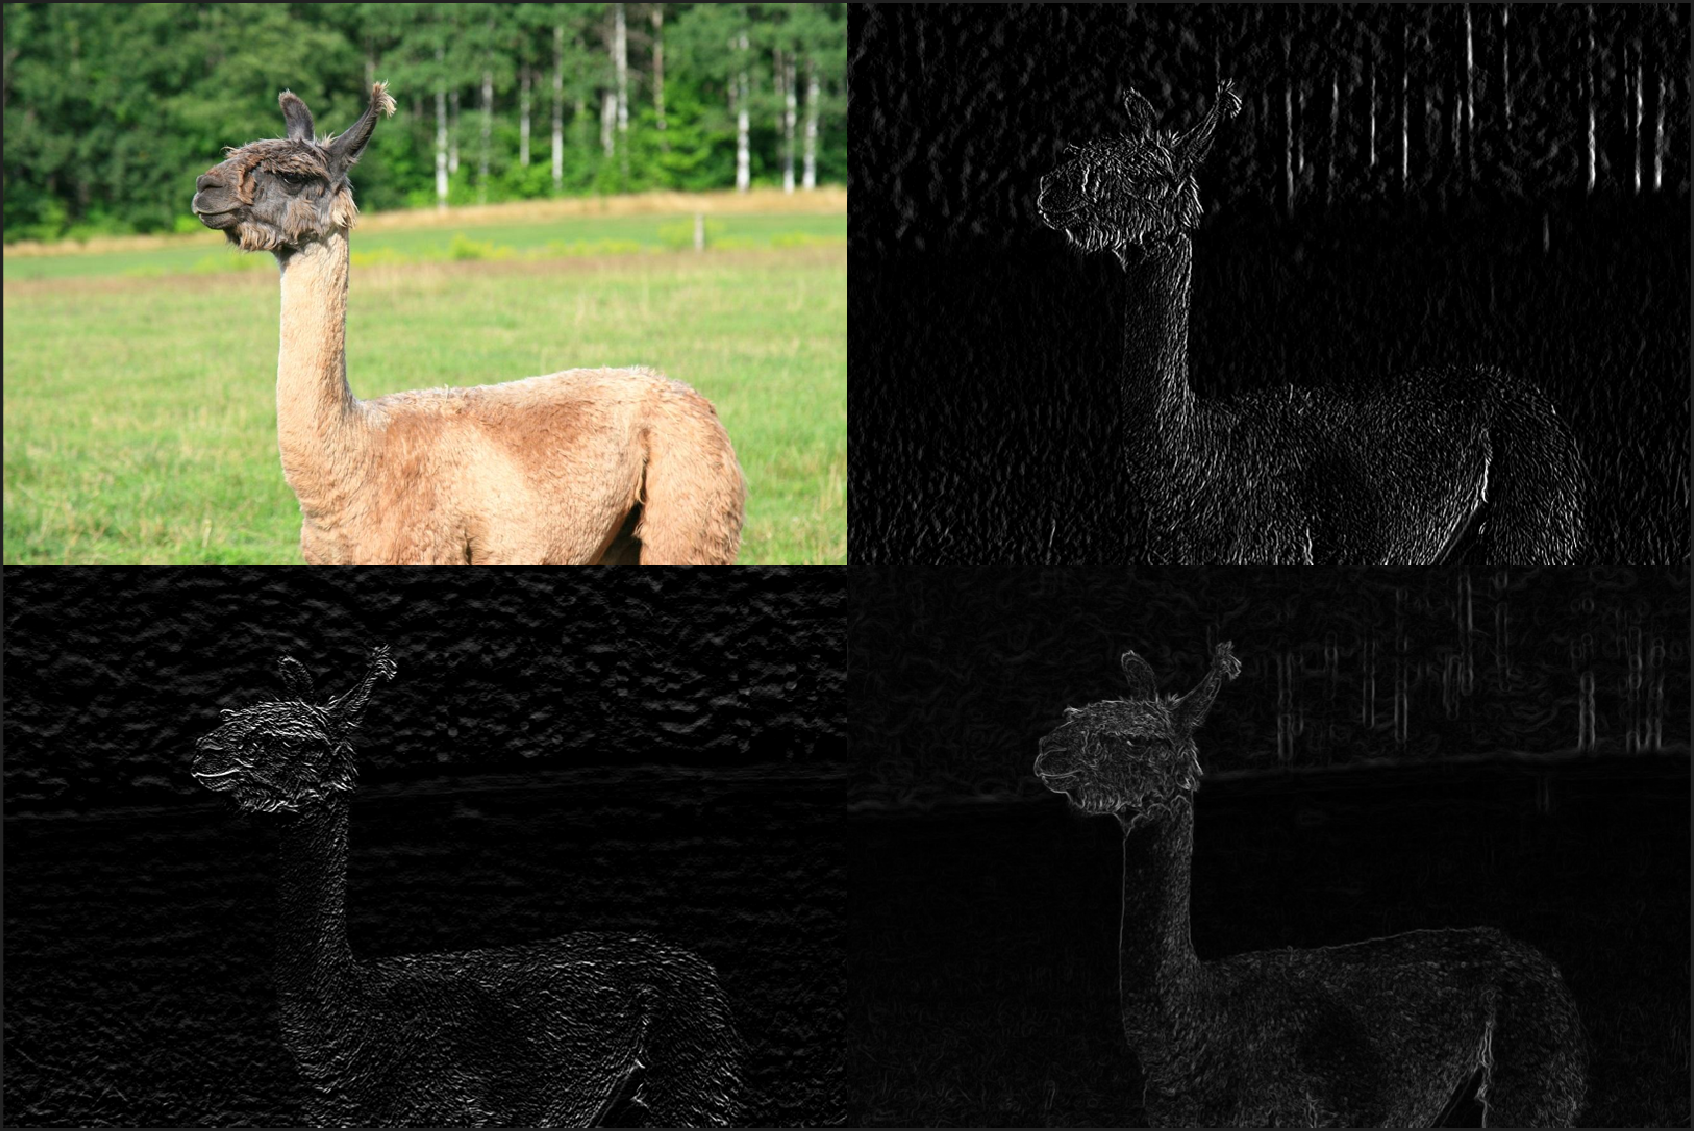
\includegraphics[scale = .4]{ejemplo_sobel}
			\caption{Detección de bordes aplicando los kernel Sobel}
			\label{fig:sobel}
		\end{figure}
		
		A continuación se va a calcular la convolución de la matriz del ejemplo anterior con $G_u$. Para verificar los cálculos, de nuevo se aplica la función \texttt{convn} de MATLAB. Al realizar los cálculos a mano tal y como se ha mostrado en el ejemplo anterior, se obtiene como resultado la matriz $A$, mientras que MATLAB devuelve la matriz $B$, esta vez los resultados no concuerdan. ¿Qué acaba de suceder? ¿Está mal codificada la función de MATLAB? ¿Está mal realizado el ejemplo?
		
		\begin{align*} A &= 
			\begin{pmatrix}
				4 & 4 & 4\\
				-4 & -4 & -4\\
				-4 & -4 & -4
			\end{pmatrix}&
			B &= \begin{pmatrix}
				-4 & -4 & -4\\
				4 & 4 & 4\\
				4 & 4 & 4
				\end{pmatrix}
		\end{align*}
		
		La respuesta a estas preguntas se podría resumir en que se ha realizado una ``pequeña trampa'' a la hora de explicar cómo calcular la convolución manualmente en el ejemplo, ya que no se ha aplicado correctamente la definición dada. ¿Qué sentido tiene hacer esto? En visión artificial y tratamiento de imágenes, muchos autores y librerías llaman convolución a la operación que se ha mostrado en el primer ejemplo, cuando en realidad no lo es y trae lugar a confusión. Dicha operación se llama correlación cruzada, denotada por $(\star)$, y que es muy similar a la convolución, pues su principal diferencia es que en la convolución ``real'', el kernel se rota 180 grados antes de calcular la convolución ``falsa'' o correlación cruzada, es decir, $X \ast Y = X \star (R_{180} \cdot Y)$, donde $R_{180}$ es la matriz de rotación de 180 grados. En el primer ejemplo se ha utilizado de manera intencionada la matriz $I_3$ para ver los casos que traen lugar a confusión, pues $I_3 \cdot R_{180} = I_3$. La correlación cruzada de dos imágenes (matrices) se define de la siguiente manera\cite{Goodfellow-et-al-2016}. 
		
		$$
		(f \star g)(u, v) = \sum_{i=-k}^{k}\sum_{j=-k}^{k} g(i, j)f(u + i, v + j)
		$$
		
		Esta operación sí es con la que realmente se aplican los filtros a las imágenes y con la que se trabaja en general en el campo de la visión artificial. Es importante ver que ahora, al contrario que con la convolución, $f \star g \neq g \star f$. Algunas librerías de visión artificial tratan a la correlación cruzada como convolución debido al frecuente uso que tiene una sobre la otra y la forma similar que tienen de calcularse. Un ejemplo es OpenCV para Python y C++ en la documentación de su función \texttt{filter2D}, donde se comenta que aplica una convolución cuando realmente aplica la correlación cruzada\cite{OpenCVFiltering}. Como se verá en próximos capítulos, las famosas redes neuronales convolucionales, no aplican convoluciones sino correlaciones cruzadas. \\
		
		Finalmenete, a la hora de realizar estas operaciones, se pueden definir una serie de parámetros según convenga para obtener un tamaño diferente de salida\cite{introCNN}. Estos son \textit{stride} y \textit{padding}. El primero de ellos hace referencia a cada cuántos elementos se desplaza el kernel y se calcula el producto escalar, mientras que el segundo a cómo rellenar los bordes de la matriz original para obtener mayor tamaño de salida, habitualmente se colocan ceros en los bordes y se conoce como \textit{zero-padding}. El tamaño de salida se puede calcular como 
		$$
		\frac{n-k+2p}{s}+1, 
		$$
		y algunos valores por defecto para el \textit{padding} son \textit{valid},  \textit{full}, y \textit{same}. Con \textit{valid} no se añade ningún \textit{padding} de manera que el kernel solo se desliza en las zonas donde la matriz de entrada y el kernel coinciden por completo, con \textit{full} se añaden las filas y columnas de ceros necesarias para poder deslizar el kernel por cualquier zona en la que coincidan la matriz y el kernel, y con \textit{same} también se añaden las necesarias como para producir un tamaño de salida igual al de entrada. A partir de ahora, cuando se utilice el parámetro \textit{full}, las operaciones se escribirán como $\circledast$ y $\ostar$, pues la definición original se entiende como \textit{valid}. En ambos casos se tomará un \textit{stride} de 1. 